\chapter{Analisis}
\label{chap:analisis}

Bab ini terdiri atas tiga bagian, yaitu Analisis CAPTCHA Yang akan Digunakan Berdasarkan Pedoman Untuk CAPTCHA, Analisis OCR yang Digunakan, dan Analisi Berorientasi Objek. Bagian Analisis CAPTCHA Yang akan Digunakan Berdasarkan Pedoman Untuk CAPTCHA berisi penjelasan analisis CAPTCHA yang akan dikembangan pada penelitian ini. Bagian Analisis OCR yang Digunakan berisi penjelasan analisis OCR yang akan digunakan pada penelitian ini. Sedangkan bagian Analisi Berorientasi Objek berisi use case diagram dan skenario perangkat lunak yang akan dibangun.

\section{Analisis CAPTCHA Yang akan Digunakan Berdasarkan Pedoman Untuk CAPTCHA}
\label{sec:analisisCAPTCHA}

Berdasarkan pedoman untuk CAPTCHA yang terdapat pada bab 2, maka beberapa hal yang akan digunakan untuk memenuhi pedoman tersebut dalam implementasi CAPTCHA pada perangkat lunak yang akan dikembangkan sebagai berikut :

\begin{enumerate}
\item
Aksesbilitas : Untuk memenuhi pedoman ini, perlu ditambah pilihan untuk CAPTCHA berbasis audio. Agar CAPTCHA tetap dapat diakses oleh orang yang memiliki gangguan pada penglihatannya. Namun pada perangkat lunak yang akan dibuat pada penelitian ini tidak menggunakan CAPTCHA berbasis audio karena tidak sesuai dengan batasan masalah.

\item
Keamanan Gambar : Untuk memenuhi pedoman ini, maka gambar yang akan dibangkitkan pada penelitian ini akan ditambah efek distorsi. Efek distorsi yang akan digunakan adalah rotasi, {\it flip}, dan {\it warp}. Ketiga efek distorsi tersebut akan dibahas pada sub bab berikut.

\item
Keamanan Skrip : Untuk menjaga keamanan skrip, maka pada pembangunan perangakat lunak ini {\it value} dari CAPTCHA yang dibangkitkan tidak akan muncul didalam skrip. Namun {\it value} masih dapat digunakan untuk memvalidasi CAPTCHA yang telah dibangkitkan. Cara yang digunakan untuk mengatasi kemanan skrip yaitu menggunakan \verb+$_SESSION+.

\item
Keamanan Tetap Terjamin Walaupun Telah Digunakan Dengan Luas : CAPTCHA yang dibangkitkan harus terjamin dari segi kualitas maupun keamanan walaupun CAPTCHA telah digunakan dengan luas. CAPTCHA yang tidak terjamin adalah CAPTCHA yang memiliki pola seperti soal matematika (penjumlahan, pengurangan, perkalian, dan pembagian). Contohnya seperti 'berapakah hasil dari 1 + 1?'. Pada penelitan ini tidak menggunakan pola yang seperti soal matematika tersebut, karena CAPTCHA yang akan dibangkitkan adalah CAPTCHA berbasis teks yang akan ditambah efek distorsi secara acak.

\item
Haruskah Membuat CAPTCHA Versi Sendiri? : Menurut pedoman yang ada, membuat CAPTCHA versi sendiri merupakan hal yang buruk. Namun hal tersebut tidak berlaku pada penelitian ini karena hasil penelitian ini tidak akan digunakan pada situs web tertentu. Dengan penelitian ini akan dibuktikan dalam pengembangan perangkat lunak bahwa membuat CAPTCHA versi sendiri tidaklah buruk, bahkan dapat menghasilkan CAPTCHA dengan kualitas yang baik.
\end{enumerate}

\subsection{Efek Rotasi Pada Karakter}
Efek rotasi pada karakter yang akan digunakan adalah rotasi dari $0^{\circ}$ sampai $360^{\circ}$ secara acak. Fungsi PHP GD yang digunakan untuk efek ini adalah
\begin{verbatim}
imagerotate ( $image , $derajat , $bgd_color )
\end{verbatim}
\verb+$image+ merupakan sumber gambar dan dikeluarkan sebagai hasil, \verb+$derajat+ merupakan parameter yang diisi $0^{\circ}$ sampai $360^{\circ}$ secara acak, \verb+$bgd_color+ merupakan parameter yang menentukan warna latar belakang yang akan menggunakan \verb+$white+ dimana \verb+$white = imagecolorallocate($image, 255, 255, 255)+. Untuk contoh penggunaan fungsi tersebut dapat dilihat pada tabel \ref{tab:rotasi}.

\begin{center}
\begin{table}
\caption[Tabel 3-1 Efek Rotasi Pada Karakter]{Efek Rotasi Pada Karakter}\\
\label{tab:rotasi}
\begin{center}
\begin{tabular}{|l|l|1|l|}
\hline
Karakter yang Diuji & Derajat & Gambar yang Diuji & Hasil OCR\\
\hline
Y & 66 & \includegraphics[scale=0.5]{Gambar/horG.png} & A.\\
\hline
2 & 102 & \includegraphics[scale=0.5]{Gambar/horm.png} & :4\\
\hline
H & 195 & \includegraphics[scale=0.5]{Gambar/hor2.png} & H\\
\hline
x & 265 & \includegraphics[scale=0.5]{Gambar/verH.png} & x\\
\hline
\end{tabular}
\end{center}
\end{table}
\end{center}

\subsection{Efek Pembalikkan Karakter}
Efek pembalikkan karakter merupakan efek yang dihasilkan dari karakter yang dibalikkan terhadap sumbu x atau sumbu y atau keduanya. Jadi seolah-olah karakter yang dihasilkan oleh efek ini seperti efek yang dihasilkan oleh cermin. Fugsi PHP GD yang digunakan untuk efek ini adalah
\begin{verbatim}
imageflip ( $image , $mode )
\end{verbatim}
\verb+$image+ merupakan sumber gambar, \verb+$mode+ merupakan parameter yang yang menentukan karakter akan dibalik terhadap horisontal (\verb+IMG_FLIP_HORIZONTAL+) atau vertikal (\verb+IMG_FLIP_VERTICAL+) atau keduanya (\verb+IMG_FLIP_BOTH+). Untuk beberapa contoh penggunaan fungsi tersebut dapat dilihat pada tabel \ref{tab:flip}.

\begin{center}
\begin{table}
\caption[Tabel 3-2 Efek Pembalikkan Karakter]{Efek Pembalikkan Karakter}\\
\label{tab:flip}
\begin{center}
\begin{tabular}{|l|l|l|}
\hline
Karakter yang Diuji & Gambar yang Diuji & Hasil OCR\\
\hline
G & \includegraphics[scale=0.5]{Gambar/horG.png} & 0\\
\hline
m & \includegraphics[scale=0.5]{Gambar/horm.png} & -\\
\hline
2 & \includegraphics[scale=0.5]{Gambar/hor2.png} & g\\
\hline
H & \includegraphics[scale=0.5]{Gambar/verH.png} & H\\
\hline
c & \includegraphics[scale=0.5]{Gambar/verc.png} & c\\
\hline
2 & \includegraphics[scale=0.5]{Gambar/ver2.png} & S\\
\hline
E & \includegraphics[scale=0.5]{Gambar/bothE.png} & 3\\
\hline
a & \includegraphics[scale=0.5]{Gambar/botha.png} & 2\\
\hline
7 & \includegraphics[scale=0.5]{Gambar/both7.png} & 4\\
\hline
\end{tabular}
\end{center}
\end{table}
\end{center}

\subsection{Menambah Efek Garis Pada Karakter}
Efek distorsi terakhir yang akan digunakan pada perangkat lunak adalah menambah efek garis pada karakter. Fungsi yang digunakan untuk efek distorsi ini adalah
\begin{verbatim}
imageline ($image, $x1, $y1, $x2, $y2, $color)
\end{verbatim}
\verb"$image" merupakan sumber gambar yang akan ditambahkan efek garis. Lalu untuk \verb"$x1" yang digunakan adalah 0 sebagai batas awal dari gambar pada sumbu x dan \verb"$x2" yang digunakan adalah 200 sebagai batas akhir dari gambar terhadap sumbu x. Dan yang terakhir untuk \verb"$y1, $y2" akan diacak dari 0 hingga 50 sebagai batas gambar awal dan akhir terhadap sumbu y. Untuk beberapa contoh penggunaan fungsi tersebut dapat dilihat pada tabel \ref{tab:line}.

\begin{center}
\begin{table}
\caption[Tabel 3-3 Efek Garis Pada Karakter]{Efek Garis Pada Karakter}\\
\label{tab:line}
\begin{center}
\begin{tabular}{|l|l|1|l|}
\hline
Karakter yang Diuji & Banyak Garis & Gambar yang Diuji & Hasil OCR\\
\hline
V & 1 & \includegraphics[scale=0.5]{Gambar/11.png} & V\\
\hline
j & 1 & \includegraphics[scale=0.5]{Gambar/12.png} & /a/\\
\hline
9 & 1 & \includegraphics[scale=0.5]{Gambar/13.png} & /\\
\hline
P & 2 & \includegraphics[scale=0.5]{Gambar/21.png} & P\\
\hline
F & 2 & \includegraphics[scale=0.5]{Gambar/22.png} & 7\\
\hline
8 & 2 & \includegraphics[scale=0.5]{Gambar/23.png} & tr\\
\hline
M & 3 & \includegraphics[scale=0.5]{Gambar/31.png} & I\\
\hline
c & 3 & \includegraphics[scale=0.5]{Gambar/32.png} & \backslash\\
\hline
Y & 3 & \includegraphics[scale=0.5]{Gambar/33.png} & V\\
\hline
\end{tabular}
\end{center}
\end{table}
\end{center}

\subsection{Mengukur Kemungkinan Kemunculan Karakter Pada CAPTCHA}
CAPTCHA yang akan dibangkitkan pada perangkat lunak yang sedang dikembangkan ini terdiri dari beberapa karakter, antara lain :

\begin{enumerate}
\item
Huruf kapital (A-Z) berjumlah 26 karakter.
\item
Huruf kecil (a-z) berjumlah 26 karakter.
\item
Angka desimal (0-9) berjumlah 10 karakter.
\end{enumerate}

Total kemungkinan karakter yang dapat digunakan pada satu karakter di CAPTCHA yang akan dibangkitkan adalah 62 karakter. Untuk menjabarkan jumlah kemungkinan karakter menggunakan kaidah perkalian, rumus yang digunakan adalah $62^n$, dimana n adalah panjang karakter yang digunakan. Penjabaran jumlah karakter, jumlah kemungkinan, dan waktu yang dibutuhkan untuk memecahkan dengan komputer yang memiliki kecepatan rata-rata 1GHz dapat dilihat pada tabel \ref{tab:kemungkinankarakter}. Kecepatan rata-rata sebuah komputer saat ini adalah 1GHZ sama dengan 1 miliar hertz atau siklus per detik. Hal tersebut berarti bahwa komputer yang memiliki kecepatan 1GHz mampu melaksanakan 1 miliar perhitungan setiap detik. Maka dari itu jumlah karakter yang akan dibangkitkan harus memiliki waktu yang cukup lama jika dipecahkan oleh komputer. Dapat dilihat jika yang jumlah karakter yang dibangkitkan adalah 1, maka waktu yang diperlukan untuk memecahkan CAPTCHA dengan panjang satu karakter yaitu $(62 / 1000000000) \times 3600 = 0.0002232$ jam. Tidak mencapai satu jam bahkan tidak memeperlukan setengah jam untuk memecahkan CAPTCHA dengan panjang satu karakter.
Untuk memenuhi keamanan, menurut penulis CAPTCHA yang akan dibangkitkan setidaknya harus memiliki minimal setengah jam untuk waktu memecahkan CAPTCHA tersebut. Dengan demikian CAPTCHA yang akan dibangkitkan minimal memiliki 3 panjang karakter.   

\begin{center}
\begin{table}
\caption[Tabel 3-4 Kemungkinan Karakter]{Kemungkinan Karakter}\\
\label{tab:kemungkinankarakter}
\begin{center}
\begin{tabular}{|l|l|1|}
\hline
Panjang Karakter & Jumlah Kemungkinan & Waktu Yang Dibutuhkan (1GHz)\\
\hline
1 & ${62}^{1} = 62$ & $0.00022$ jam\\
\hline
2 & ${62}^{2} = 3.84 \times 10^3$ & $0.01383$ jam\\
\hline
3 & ${62}^{3} = 2.38 \times 10^5$ & $0.85798$ jam\\
\hline
4 & ${62}^{4} = 1.47 \times 10^7$ & $53.19480$ jam\\
\hline
5 & ${62}^{5} = 9.16 \times 10^8$ & $32.98078 \times 10^{2}$ jam\\
\hline
6 & ${62}^{6} = 5.68 \times 10^{10}$ & $20.44808 \times 10^{4}$ jam\\
\hline
7 & ${62}^{7} = 3.52 \times 10^{12}$ & $12.67781 \times 10^{6}$ jam\\
\hline
8 & ${62}^{8} = 2.18 \times 10^{14}$ & $78.60243 \times 10^{7}$ jam\\
\hline
9 & ${62}^{9} = 1.35 \times 10^{16}$ & $48.73351 \times 10^{9}$ jam\\
\hline
10 & ${62}^{10} = 8.39 \times 10^{18}$ & $30.21477 \times 10^{11}$ jam\\
\hline
11 & ${62}^{11} = 5.20 \times 10^{19}$ & $18.73316 \times 10^{13}$ jam\\
\hline
12 & ${62}^{12} = 3.22 \times 10^{21}$ & $11.61456 \times 10^{15}$ jam\\
\hline
13 & ${62}^{13} = 2 \times 10^{23}$ & $72.01027 \times 10^{16}$ jam\\
\hline
14 & ${62}^{14} = 1.24 \times 10^{25}$ & $44.64636 \times 10^{18}$ jam\\
\hline
15 & ${62}^{15} = 7.68 \times 10^{26}$ & $27.68074 \times 10^{20}$ jam\\
\hline
\end{tabular}
\end{center}
\end{table}
\end{center}

\section{Analisis OCR yang Digunakan}
\label{sec:analisisOCR}

Dari beberapa perangkat lunak OCR yang terdapat pada bab 2. Perangkat lunak OCR yang dipilih untuk mengukur kualitas CAPTCHA adalah Tesseract OCR. Tesseract OCR dipilih karena merupakan perangkat lunak open source yang memiliki lisensi Apache versi 2.0 dan disponsori oleh Google. Alasan utama memilih Tesseract OCR karena adanya lisensi Apache yang akan menunjang penelitian ini yang berbasis PHP. Tesseract OCR dianggap sebagai salah satu perangkat lunak OCR yang paling akurat untuk saat ini.

\section{Analisis Berorientasi Objek}
\label{sec:analisisberorientasiobjek}

Pembahasan use case diagram, skenario, dan modul yang akan digunakan pada penelitian.

\subsection{Use Case Diagram}
\begin{figure}[H]
\centering
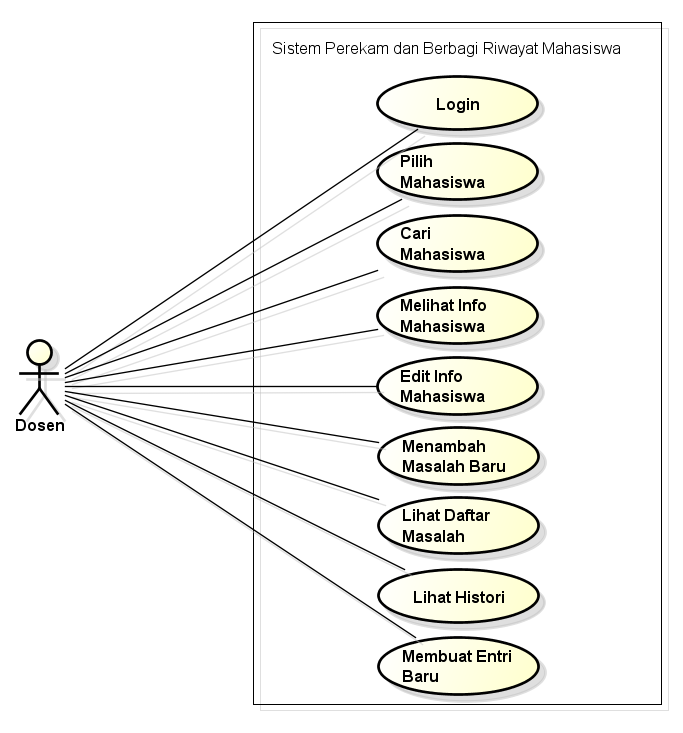
\includegraphics[scale=1]{Gambar/usecase.jpg}
\caption[Use Case Diagram]{Use Case Diagram} 
\label{fig:usecase}
\end{figure}

Use case diagram merupakan pemodelan yang menunjukkan kegiatan apa saja yang dapat dilakukan pengguna dan kegiatan yang dilakukan sistem. Berikut adalah deskripsi dari use case pada gambar \ref{fig:usecase}.

\begin{itemize}
\item Menguji CAPTCHA
Use case ini memungkinkan pengguna dapat menguji CAPTCHA yang dibangkitkan secara otomatis secara langsung.
\item Menguji dengan OCR
Use case ini memungkinkan perangkat lunak untuk melakukan pengujian CAPTCHA dengan OCR secara otomatis.
\item Melihat hasil
Use case ini memungkinkan pengguna untuk melihat hasil setelah melakukan pengujian terhadap CAPTCHA baik dari pengujian yang dilakukannya maupun hasil pengujian dengan OCR.
\end{itemize}

\subsection{Skenario}
\subsubsection{Menguji CAPTCHA}

\begin{table}
\centering
\caption[Tabel 3-5 Skenario Menguji CAPTCHA]{Skenario Menguji CAPTCHA}
\label{tab:skenariomengujicaptcha}
\begin{tabular}{|p{1.4cm}|p{0.4cm}|p{2cm}|p{2cm}|p{2cm}|p{2cm}|}
\hline
Nama & \multicolumn{5}{p{8cm}|}{Menguji CAPTCHA} \\ \hline
Aktor & \multicolumn{5}{p{8cm}|}{User} \\ \hline
Deskripsi & \multicolumn{5}{p{8cm}|}{Menguji CAPTCHA yang dibangkitkan secara otomatis} \\ \hline
Kondisi Awal & \multicolumn{5}{p{8cm}|}{Belum ada gamabar CAPTCHA yang dibangkitkan} \\ \hline
Kondisi Akhir & \multicolumn{5}{p{8cm}|}{Hasil jawaban user ditampilkan beserta keterangan benar atau salah} \\ \hline
\multirow{Skenario Utama} & No & \multicolumn{2}{p{4cm}|}{Aksi Aktor} & \multicolumn{2}{p{4cm}|}{Reaksi Sistem} \\ \cline{2-6} 
 & 1 & \multicolumn{2}{p{4cm}|}{Aktor harus memilih panjang karakter yang akan diuji} & \multicolumn{2}{p{4cm}|}{Sistem akan menampilkan pilihan untuk panjang karakter} \\ \cline{2-6} 
 & 2 & \multicolumn{2}{p{4cm}|}{Aktor mengklik panjang karakter yang akan dipilih} & \multicolumn{2}{p{4cm}|}{Sistem akan membangkitkan gambar CAPTCHA secara otomatis} \\ \cline{2-6} 
 & 3 & \multicolumn{2}{p{4cm}|}{Aktor memasukan jawaban dari gambar CAPTCHA} & \multicolumn{2}{p{4cm}|}{Sistem akan memeriksa jawaban dari user} \\ \hline
Eksepsi & \multicolumn{5}{p{8cm}|}{-} \\ \hline
\end{tabular}
\end{table}

%\begin{center}
%\begin{table}
%\caption[Tabel 3-6 Skenario Menguji CAPTCHA]{Tabel 3-6 Skenario %Menguji CAPTCHA}\\
%\begin{center}
%\begin{tabular}{|l|l|l|l|l|l|}
%\hline
%Nama & \multicolumn{5}{l|}{Menguji CAPTCHA} \\ \hline
%Aktor & \multicolumn{5}{l|}{User} \\ \hline
%Deskripsi & \multicolumn{5}{l|}{Menguji CAPTCHA yang dibangkitkan secara otomatis} \\ \hline
%Kondisi Awal & \multicolumn{5}{l|}{Belum ada gamabar CAPTCHA yang dibangkitkan} \\ \hline
%Kondisi Akhir & \multicolumn{5}{l|}{Hasil jawaban user ditampilkan beserta keterangan benar atau salah} \\ \hline
%\multirow{Skenario Utama} & No & \multicolumn{2}{l|}{Aksi Aktor} & \multicolumn{2}{l|}{Reaksi Sistem} \\ \cline{2-6} 
% & 1 & \multicolumn{2}{l|}{Aktor harus memilih panjang karakter yang akan diuji} & \multicolumn{2}{l|}{Sistem akan menampilkan pilihan-pilihan untuk panjang karakter} \\ \cline{2-6} 
% & 2 & \multicolumn{2}{l|}{Aktor mengklik panjang karakter yang akan dipilih} & \multicolumn{2}{l|}{Sistem akan membangkitkan gambar CAPTCHA secara otomatis} \\ \cline{2-6} 
% & 3 & \multicolumn{2}{l|}{Aktor memasukan jawaban dari gambar CAPTCHA} & \multicolumn{2}{l|}{Sistem akan memeriksa jawaban dari user} \\ \hline
%Eksepsi & \multicolumn{5}{l|}{-} \\ \hline
%\end{tabular}
%\end{center}
%\end{table}
%\end{center}

Untuk use case \textquotedblleft Menguji CAPTCHA\textquotedblleft, skenarionya dapat dilihat pada Tabel \ref{tab:skenariomengujicaptcha}.

\subsubsection{Menguji dengan OCR}

\begin{table}
\centering
\caption[Tabel 3-6 Skenario Menguji dengan OCR]{Skenario Menguji dengan OCR}
\label{tab:skenariomengujicaptchadenganocr}
\begin{tabular}{|p{1.4cm}|p{0.4cm}|p{2cm}|p{2cm}|p{2cm}|p{2cm}|}
\hline
Nama & \multicolumn{5}{p{8cm}|}{Menguji dengan OCR} \\ \hline
Aktor & \multicolumn{5}{p{8cm}|}{Komputer} \\ \hline
Deskripsi & \multicolumn{5}{p{8cm}|}{Menguji CAPTCHA yang dibangkitkan dengan OCR secara otomatis} \\ \hline
Kondisi Awal & \multicolumn{5}{p{8cm}|}{Gambar CAPTCHA yang telah dibangkitkan} \\ \hline
Kondisi Akhir & \multicolumn{5}{p{8cm}|}{Hasil jawaban OCR ditampilkan beserta keterangan benar atau salah} \\ \hline
\multirow{Skenario Utama} & No & \multicolumn{2}{p{4cm}|}{Aksi Aktor} & \multicolumn{2}{p{4cm}|}{Reaksi Sistem} \\ \cline{2-6} 
 & 1 & \multicolumn{2}{p{4cm}|}{Gambar CAPTCHA yang dibangkitkan diambil untuk dipecahkan} & \multicolumn{2}{p{4cm}|}{Sistem akan mengambil gambar CAPTCHA dan menguji dengan OCR} \\ \cline{2-6} 
 & 2 & \multicolumn{2}{p{4cm}|}{Gambar CAPTCHA akan diproses dengan OCR} & \multicolumn{2}{p{4cm}|}{Sistem akan mendapatkan jawaban CAPTCHA dari OCR} \\ \cline{2-6} 
 & 3 & \multicolumn{2}{p{4cm}|}{Komputer akan mengambil jawaban CAPTCHA dari OCR} & \multicolumn{2}{p{4cm}|}{Sistem akan menampilkan dan memeriksa jawaban dari OCR} \\ \hline
Eksepsi & \multicolumn{5}{p{8cm}|}{-} \\ \hline
\end{tabular}
\end{table}

Untuk use case \textquotedblleft Menguji dengan OCR\textquotedblleft, skenarionya dapat dilihat pada Tabel \ref{tab:skenariomengujicaptchadenganocr}.

\subsubsection{Melihat Hasil}


\begin{table}
\centering
\caption[Tabel 3-7 Skenario Melihat hasil]{Skenario Melihat hasil}
\label{tab:skenariomelihathasil}
\begin{tabular}{|p{1.4cm}|p{0.4cm}|p{2cm}|p{2cm}|p{2cm}|p{2cm}|}
\hline
Nama & \multicolumn{5}{p{8cm}|}{Melihat Hasil} \\ \hline
Aktor & \multicolumn{5}{p{8cm}|}{User} \\ \hline
Deskripsi & \multicolumn{5}{p{8cm}|}{Melihat hasil pengujian CAPTCHA dari sisi user dan komputer} \\ \hline
Kondisi Awal & \multicolumn{5}{p{8cm}|}{Menampilkan tabel untuk memuat data hasil uji} \\ \hline
Kondisi Akhir & \multicolumn{5}{p{8cm}|}{Hasil jawaban user dan komputer ditampilkan dalam tabel beserta isi, tebakan, jawaban, dan keterangan} \\ \hline
\multirow{Skenario Utama} & No & \multicolumn{2}{p{4cm}|}{Aksi Aktor} & \multicolumn{2}{p{4cm}|}{Reaksi Sistem} \\ \cline{2-6} 
 & 1 & \multicolumn{2}{p{4cm}|}{Aktor selesai menjalankan menguji CAPTCHA dan telah melewati menguji dengan OCR} & \multicolumn{2}{p{4cm}|}{Sistem akan menampilkan tabel hasil} \\ \hline
Eksepsi & \multicolumn{5}{p{8cm}|}{-} \\ \hline
\end{tabular}
\end{table}

Untuk use case \textquotedblleft Melihat hasil\textquotedblleft, skenarionya dapat dilihat pada Tabel \ref{tab:skenariomelihathasil}.
